\documentclass[UTF8]{article}
\usepackage{graphicx}
\usepackage{subfigure}
\usepackage{amsmath}
\usepackage{makecell}
\usepackage[utf8]{inputenc}
\usepackage[space]{ctex} %中文包
\usepackage{listings} %放代码
\usepackage{xcolor} %代码着色宏包
\usepackage{CJK} %显示中文宏包
\usepackage{float}
\usepackage{makecell}
\usepackage{diagbox}
\usepackage{bm}
\usepackage{ulem} 
\usepackage{amssymb}
\usepackage{soul}
\usepackage{color}
\usepackage{geometry}
\usepackage{fancybox} %花里胡哨的盒子
\usepackage{xhfill} %填充包, 可画分割线 https://www.latexstudio.net/archives/8245
\usepackage{multicol} %多栏包
\usepackage{enumerate} %可以方便地自定义枚举标题
\usepackage{multirow} %表格中多行单元格合并
\usepackage{wasysym} %可以使用wasysym里的一堆奇奇怪怪的符号
\usepackage[marginal]{footmisc} % 注脚, 且不缩进

\geometry{left = 2.5cm, right = 2.5cm, bottom = 2.5cm, top = 2.5cm}

\definecolor{mygreen}{rgb}{0,0.6,0}
\definecolor{mygray}{rgb}{0.5,0.5,0.5}
\definecolor{mymauve}{rgb}{0.58,0,0.82}

\lstset{
	backgroundcolor=\color{white}, 
	%\tiny < \scriptsize < \footnotesize < \small < \normalsize < \large < \Large < \LARGE < \huge < \Huge
	basicstyle = \scriptsize,       
	breakatwhitespace = false,        
	breaklines = true,                 
	captionpos = b,                    
	commentstyle = \color{mygreen}\bfseries,
	escapeinside=``,
	extendedchars = false,
	frame = shadowbox, 
	framerule=0.5pt,
	keepspaces=true,
	keywordstyle=\color{blue}\bfseries, % keyword style
	language = verilog,                     % the language of code
	otherkeywords={string}, 
	numbers=left, 
	numbersep=5pt,
	numberstyle=\tiny\color{mygray},
	rulecolor=\color{black},         
	showspaces=false,  
	showstringspaces=false, 
	showtabs=false,    
	stepnumber=1,         
	stringstyle=\color{mymauve},        % string literal style
	tabsize=4,          
	title=\lstname,
	texcl=true  
}

%\sum\nolimits_{j=1}^{M}   上下标位于求和符号的水平右端,
%\sum\limits_{j=1}^{M}   上下标位于求和符号的上下处,
%\sum_{j=1}^{M}  对上下标位置没有设定,会随公式所处环境自动调整。

%%%%%%%%%%%%%画图包%%%%%%%%%%%%%
\usepackage{tikz}
%%%%%%%%%%%%%画图背景包%%%%%%%%%%%%%
\usetikzlibrary{backgrounds}

%%%%%%%%%%%%%在tikz中画一个顶点%%%%%%%%%%%%%
%%%%%%%%%%%%%#1:node名称%%%%%%%%%%%%%
%%%%%%%%%%%%%#2:位置%%%%%%%%%%%%%
%%%%%%%%%%%%%#3:标签%%%%%%%%%%%%%
\newcommand{\newVertex}[3]{\node[circle, draw=black, line width=1pt, scale=0.8] (#1) at #2{#3}}
%%%%%%%%%%%%%在tikz中画一条边%%%%%%%%%%%%%
\newcommand{\newEdge}[2]{\draw [black,very thick](#1)--(#2)}
%%%%%%%%%%%%%在tikz中放一个标签%%%%%%%%%%%%%
%%%%%%%%%%%%%#1:名称%%%%%%%%%%%%%
%%%%%%%%%%%%%#2:位置%%%%%%%%%%%%%
%%%%%%%%%%%%%#3:标签内容%%%%%%%%%%%%%
\newcommand{\newLabel}[3]{\node[line width=1pt] (#1) at #2{#3}}

%%%%%%%%%%%%%强制跳过一行%%%%%%%%%%%%%
\newcommand{\jumpLine} {\hspace*{\fill} \par}
%%%%%%%%%%%%%关键点指令,可用itemise替代%%%%%%%%%%%%%
\newcommand{\average}[1]{\left\langle #1\right\rangle }
%%%%%%%%%%%%%表格内嵌套表格%%%%%%%%%%%%%

\newcommand{\keypoint}[2]{$\bullet$\textbf{#1}\quad#2\par}
%%%%%%%%%%%%%<T>平均值表示%%%%%%%%%%%%%
\newcommand{\tabincell}[2]{\begin{tabular}{@{}#1@{}}#2\end{tabular}}%放在导言区
%%%%%%%%%%%%%大黑点item头%%%%%%%%%%%%%
\newcommand{\itemblt}{\item[$\bullet$]}
%%%%%%%%%%%%%大圈item头%%%%%%%%%%%%%
\newcommand{\itemc}{\item[$\circ$]}
%%%%%%%%%%%%%大星星item头%%%%%%%%%%%%%
\newcommand{\itembs}{\item[$\bigstar$]}
%%%%%%%%%%%%%右▷item头%%%%%%%%%%%%%
\newcommand{\itemrhd}{\item[$\rhd$]}
%%%%%%%%%%%%%定义为%%%%%%%%%%%%%
\newcommand{\defas}{=_{df}}
%%%%%%%%%%%%%蕴含%%%%%%%%%%%%%
\newcommand{\imp}{\rightarrow}

%%%%%%%%%%%%%双线分割线%%%%%%%%%%%%%
\newcommand*{\doublerule}{\hrule width \hsize height 1pt \kern 0.5mm \hrule width \hsize height 2pt}
%%%%%%%%%%%%%双线中间可加东西的分割线%%%%%%%%%%%%%
\newcommand\doublerulefill{\leavevmode\leaders\vbox{\hrule width .1pt\kern1pt\hrule}\hfill\kern0pt }
%%%%%%%%%%%%%左大括号%%%%%%%%%%%%%
\newcommand{\leftbig}[1]{\left\{\begin{array}{l}#1\end{array}\right.}
%%%%%%%%%%%%%矩阵%%%%%%%%%%%%%
\newcommand{\mat}[2]{\left[\begin{array}{#1}#2\end{array}\right]}
%%%%%%%%%%%%%可换行圆角文本框%%%%%%%%%%%%%
\newcommand{\ovalboxn}[1]{\ovalbox{\tabincell{l}{#1}}}
%%%%%%%%%%%%%设置section的counter, 使从0开始%%%%%%%%%%%%%
\setcounter{section}{0}

\title{计算机组成原理实验 实验报告}
\date{}

\begin{document}
%%%%%%%%%%%%%科大报告封面%%%%%%%%%%%%%
\maketitle
\begin{figure}[H]
	\centering
	
\includegraphics[width=2.5in]{xiaohui.png}\vspace{0.5cm}\\
	\large{
		实验题目:Lab6 综合设计\\
		学生姓名:王章瀚\\
		学生学号:PB18111697\\
		完成日期:\today\\
	}\vspace{2cm}
	
	\large{计算机实验教学中心制\\2019年09月\\}
	\thispagestyle{empty}
	\clearpage  % 清除当页页码
\end{figure}
\newpage

\section{实验题目}
Lab6 综合设计

\section{实验目的}
\begin{enumerate}
	\item 理解计算机系统的组成结构和工作原理;
	\item 理解计算机总线和接口的结构和功能;
	\item 掌握软硬件综合系统的设计和调试方法.QQQ
	
\end{enumerate}

\section{实验平台}
Vivado

\section{实验设计内容说明}
本次实验要求实现一个简单的计算机应用系统. 但其实要做好这么一个简易系统, 主要是要实现总线. \textbf{只要实现了总线, 其他更为复杂的操作, 就变成了搭积木一样简单了}. 因此认为, 讲义给出的斐波那契数列应用, 足以反映我对于总线的认识与实现它的能力. 因此就按照老师给出的应用来完成本次实验.\par
本次设计中, 采用了Lab5中完成的流水线CPU来做. 除了添加了总线设计以外, 还添加了分支预测, 便于日后实验其他功能的时候使用. 总体而言, 是设计了一个\textbf{带分支预测和总线的流水线CPU}.

\section{实验过程}
\subsection{基本过程}
\subsubsection{总线的设计}
总线的设计中, 主要需要有一个总线控制器来控制数据传输. 而相关的总线大致需要有:
\begin{enumerate}
	\item din: CPU传到总线上的数据线
	\item dout: 总线传给CPU的数据线
	\item done: 总线上din放好数据的信号
	\item we: 设备写使能
	\item re: 设备读使能
\end{enumerate}
\subsubsection{分支预测的设计}
这里分支预测采用的是2位动态分支预测, 这种预测方法足以适配大多数情况的分支预测, 实现CPU的高效性.
\subsection{数据通路}
分支预测的数据通路很简单, 就是添加了一个分支预测模块及预测是否分支的控制线等, 故这里就不展示了.\par
至于总线的数据通路和老师的没有太大区别, 但我用了自己的变量名称, 方便助教查看程序的时候能够理解.
\begin{figure}[H]
	\centering
	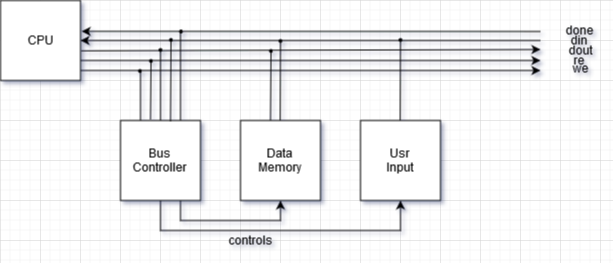
\includegraphics[width=\linewidth]{data_path.png}
	\label{data_path}
\end{figure}
\subsection{状态转换}
\subsubsection{用户输入器的状态转换}
总线控制这块没有什么太多的状态可言. 所以就简单描述一下用户Input模块的状态.\par
下面这个图描述的是需要lw到用户输入的时候, 就会阻塞等待用户输入, 知道用户按了enter(某个按钮), 才会继续.\par
\begin{figure}[H]
	\centering
	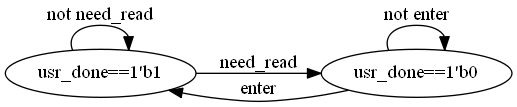
\includegraphics[width=\linewidth/3*2]{phase_diagram.png}
	\label{phase_diagram}
\end{figure}
\subsubsection{分支预测器的状态转换}
\begin{figure}[H]
	\centering
	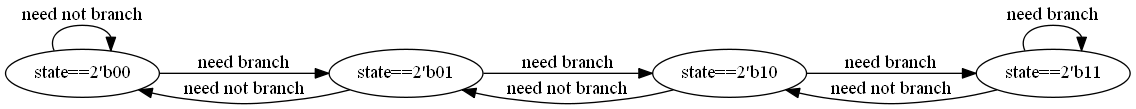
\includegraphics[width=\linewidth]{predictor_phase_diagram.png}
	\label{predictor_phase_diagram}
\end{figure}
\subsection{代码讲解}
\subsubsection{总线的代码讲解}
这里面用了两个外设, 一个是数据存储器, 另一个是自己实现的用户输入器(获取由switches表示的数据, 按某个按钮确认输入), 分别作为外设0和外设1.
这里主要需要控制的是,
\begin{enumerate}
	\item 当对应外设准备好数据的时候, done就会被置为1'b1
	\item 当对应外设未被选中, 应当作为32'hzzzz\_zzzz
	\item 当对应外设被选中, 将其输出作为总线输出(即din)
\end{enumerate}
\begin{lstlisting}[language=verilog]
module bus_unit
(
input clk,
input rst,
input [31:0] addr,
input [31:0] dout,      // CPU输出到总线的数据
input we,
input re,               // 读使能
// input of usr\_input
input enter,
input [15:0] sw,
// ouput
output [31:0] din,      // 总线要给CPU的数据
output reg done,             // done标志
input [31:0] DBU_mem_rf_addr,
output [31:0] DBU_mem_data
);

// 片选使能 addr[31:10] == en[21:0]
// 片内地址 addr[9:2]

wire [31:0] data_0;
wire [31:10] en;

assign en = addr[31:10];

// 外设0: 数据存储器
data_mem_256x32 data_mem(.a(addr >> 2),
                         .d(dout),
                         .dpra(DBU_mem_rf_addr),
                         .clk(clk),
                         .we(we),
                         .spo(data_0),
                         .dpo(DBU_mem_data));
assign din = en == 22'h0 ? data_0 : 32'hzzzz_zzzz;

// 外设1: 用户输入读取
wire [31:0] data_1;
wire usr_done;
reg need_usr_input;
wire flag;
assign flag =usr_done && need_usr_input;

usr_input usr_input(clk, rst,
                    addr[3:2],
                    re,
                    enter,
                    sw,
                    data_1,
                    usr_done);
assign din = en == 22'h1 ? data_1 : 32'hzzzz_zzzz;
                    

always @(*) begin
    case(en)
        22'h0: begin
            done = 1'b1;
        end
        22'h1: begin
            done = usr_done;
        end
        default: done = 1'b1;
    endcase
end

endmodule
\end{lstlisting}
\subsubsection{用户输入器的代码讲解}
这里输入信号需要有sw和enter(作为确认输入)\par
主要实现的内容有:
\begin{enumerate}
	\item 对enter取边沿, 以防连续输入.
	\item 在需要用户输入的时候(need\_usr\_input==1'b1), 若未摁enter, 则置done为1'b0
	\item 若用户摁了enter, 则置done为1'b1, 表示完成用户输入的读入.
\end{enumerate}
\begin{lstlisting}[language=verilog]
module usr_input
(
input clk,
input rst,
input [1:0] addr,
input need_usr_input,
input enter,
input [15:0] sw,
output reg [31:0] data,
output reg done
);

wire enter_edge;

edge_taker #(.N(1))
    input_edge_taker(.clk(clk),
                     .rst(rst),
                     .in(enter),
                     .out(enter_edge));
                     
always @(*) begin
    case(addr)
        2'b00: data = {{24{1'b0}}, sw[7:0]};
        2'b01: data = {{24{1'b0}}, sw[15:8]};
        2'b10: data = 32'hffff_ffff;
        default: data = 32'h0000_0000;
    endcase
end

always @(*) begin
    if(rst) begin
        done = 1'b1;
    end
    else begin
        if(need_usr_input) done = 1'b0;
        else done = done;
        if(enter_edge) begin
            done = 1'b1;
        end
    end
end

endmodule
\end{lstlisting}
\subsubsection{分支预测器的代码讲解}
这一部分的代码实现了一个简单的2位动态分支预测器. 代码内容主要是对分支成功与失败的时候, 作相应位的增减. 并且给出shall\_branch来告诉CPU是否预测为要分支.
\begin{lstlisting}[language=verilog]
module branch_predictor
#(
parameter HIGH = 5    // 分支预测器cache地址最高位
)
(
input clk,
input rst, 
input [5:0] im_instr_opcode,
input [HIGH:0] im_instr_lowpc,
input [HIGH:0] IF_ID_lowpc,
input IF_ID_is_branch,
input equal,
output shall_branch
);

localparam BEQ_op = 6'b000100;
localparam CACHE_SIZE = {2'b10, {HIGH{1'b0}}}; // 根据 HIGH 判断缓存大小
reg [1:0] cache[CACHE_SIZE-1:0];
integer i;

assign shall_branch = cache[im_instr_lowpc] >= 2'b10 && im_instr_opcode == BEQ_op ? 1'b1 : 1'b0;

always @(posedge clk, posedge rst) begin
    if(rst) begin
        for(i = 0; i < CACHE_SIZE; i = i + 1) begin
            cache[i] <= 2'b00;
        end
    end
    else if(IF_ID_is_branch) begin
        case(equal)
            1'b0: cache[IF_ID_lowpc] <= cache[IF_ID_lowpc] == 2'b00 ? 2'b00 : cache[IF_ID_lowpc] - 2'b01;
            1'b1: cache[IF_ID_lowpc] <= cache[IF_ID_lowpc] == 2'b11 ? 2'b11 : cache[IF_ID_lowpc] + 2'b01;
            default: cache[IF_ID_lowpc] <= 2'b01;
        endcase
    end
end

endmodule
\end{lstlisting}
\section{实验结果}
实验结果分两部分说明, 一部分是总线这一块, 另一部分是分支预测器这一块.
\subsection{总线的实验结果}
这一部分的实验验证, 采用了一个可以获取用户输入初始两个数的斐波那契数生成器, 并且在用户摁下按钮的时候, 才显示下一个数字(按照代码, 应该会显示在数码管上, 然而没有板子去验证)
\subsubsection{起始输入及第一个数计算}
可以看到下图,
\begin{enumerate}
	\item 仿真代码中将SW设置成了输入是两个1, 因此斐波那契初始值为1, 1
	\item 蓝色波形都是关于总线的波形, 标识出来方便助教查看
	\item 红色框是两个用户的enter, 标识用户确认输入的两个数字
	\item 红色框同一行后面还有一个enter, 标识用户确认显示下一个斐波那契数
	\item 紫色框是斐波那契数的sw以及在数码管将要显示的数字, 可以看到取得了1+1=2
\end{enumerate}
\begin{figure}[H]
	\centering
	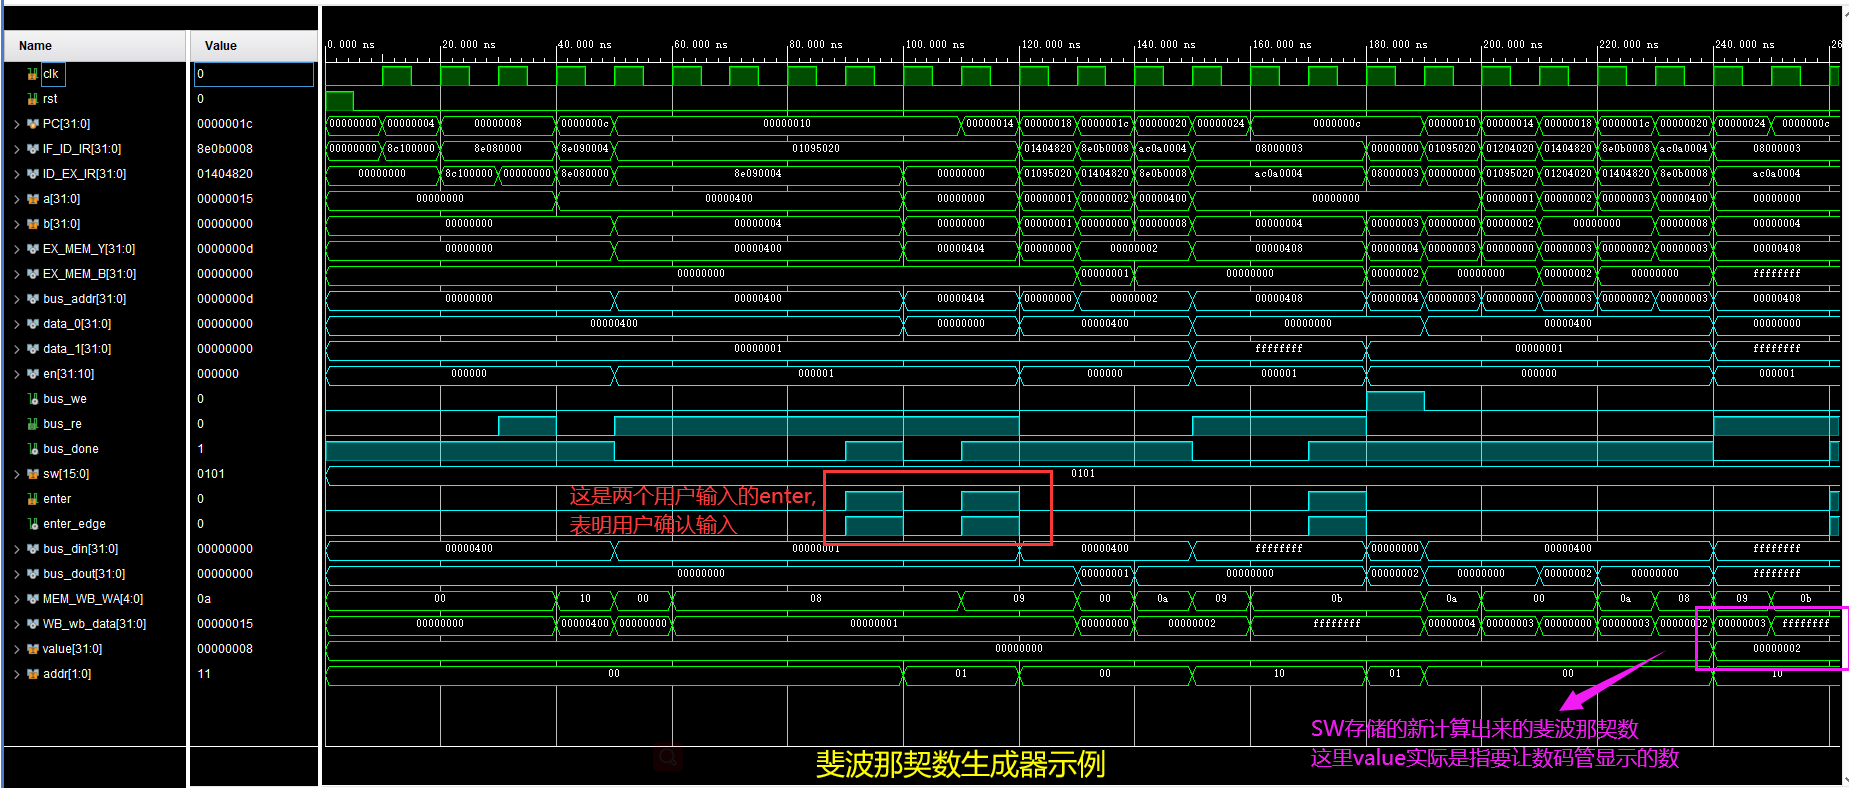
\includegraphics[width=\linewidth]{fibonacci_sample.png}
	\label{fibonacci_sample}
\end{figure}
\subsubsection{后续计算及显示}
再去看后面的数字, 也都在相应的enter后, 显示正确数字
\begin{figure}[H]
	\centering
	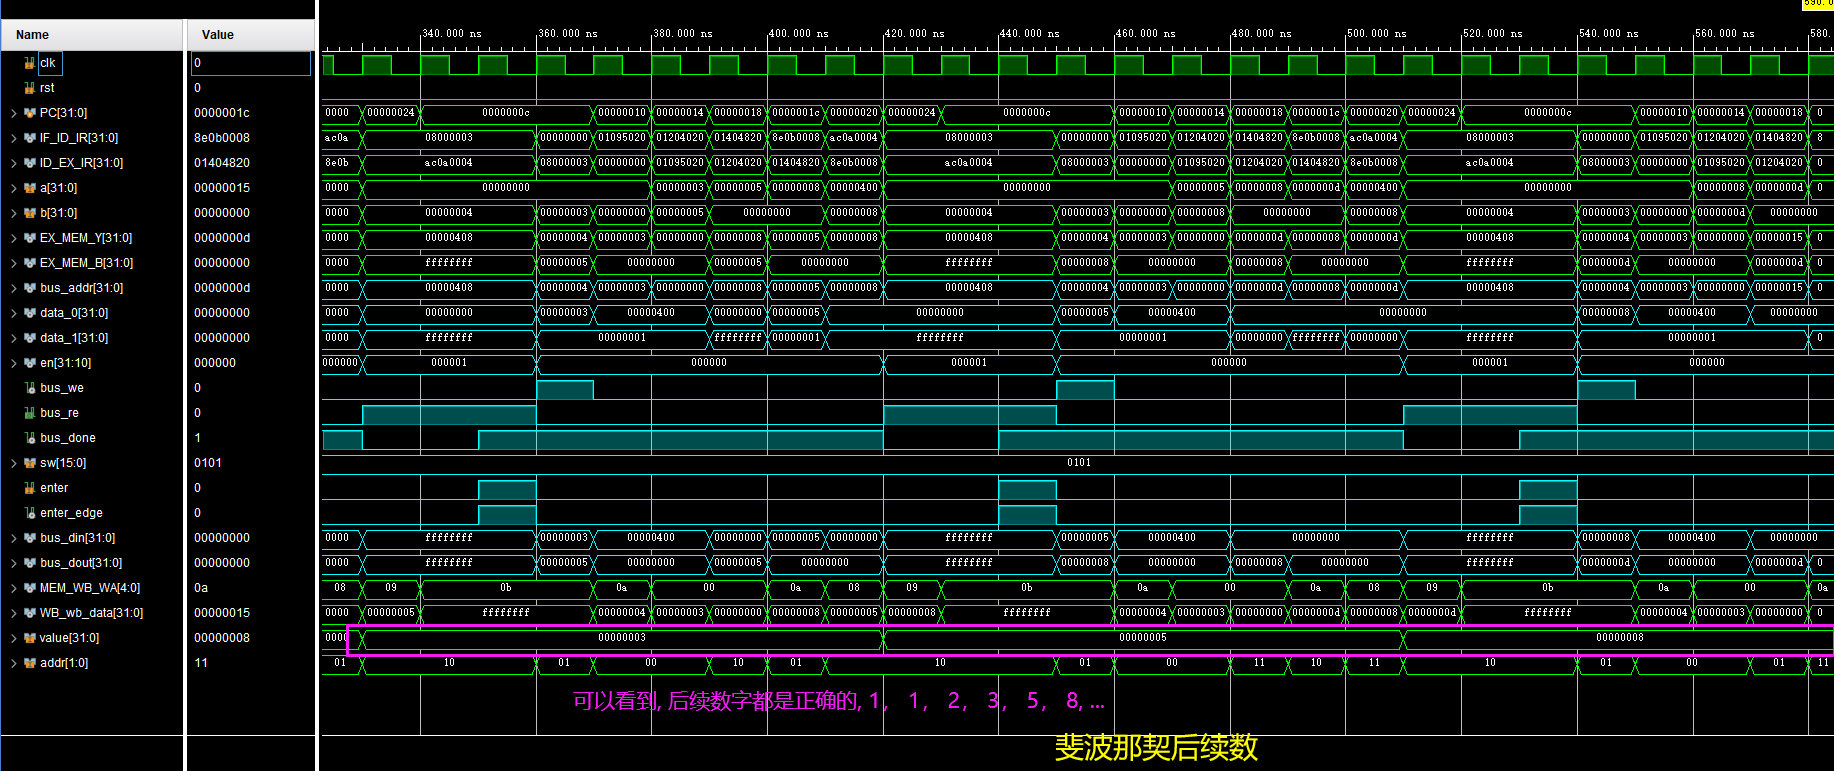
\includegraphics[width=\linewidth]{fibonacci_sequence.png}
	\label{fibonacci_sequence}
\end{figure}

\subsection{分支预测器的实验结果}
之前的代码都表现不出来分支预测有无的区别, 下面用一个能表现出区别的示例代码(见附录\ref{asm_predictor}\footnote{特别感谢黄致远同学提供分支预测的测试代码})来展现.\par
\begin{figure}[H]
	\centering
	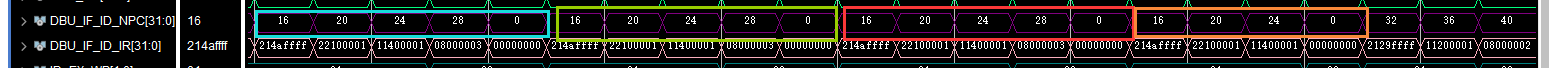
\includegraphics[width=\linewidth]{predictor.png}
\end{figure}
可以看到图中原来一个循环中IF.ID\_NPC是要经历16,20,24,28,0的循环, 过了几次后, 变成16,20,24,0了.\par
反过来也是可以的, 但是限于篇幅就不展示了, 助教如果感兴趣可以自己运行一下我的代码(附件里都有)


\section{心得体会}
有了总线的设计了, 这个系列实验下来才算比较完整. 这套实验让我学会了如何从0去搭建一个CPU, 及其配套总线等等, 收获非常大.
\section{意见建议}
没有什么意见建议.
\section{附录}
\subsection{附录1, 总线测试代码}
\begin{figure}[H]
	\centering
	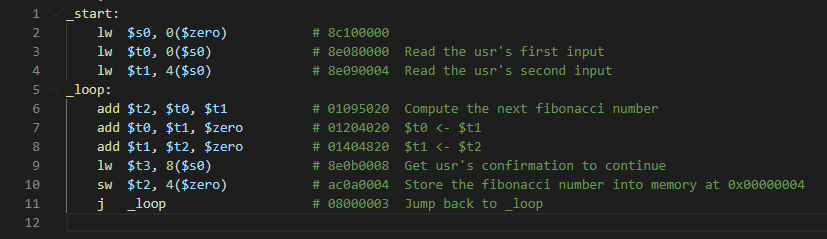
\includegraphics[width=\linewidth]{asm.png}
	\label{asm}
\end{figure}
\subsection{附录2, 分支预测器测试代码}
\begin{figure}[H]
	\centering
	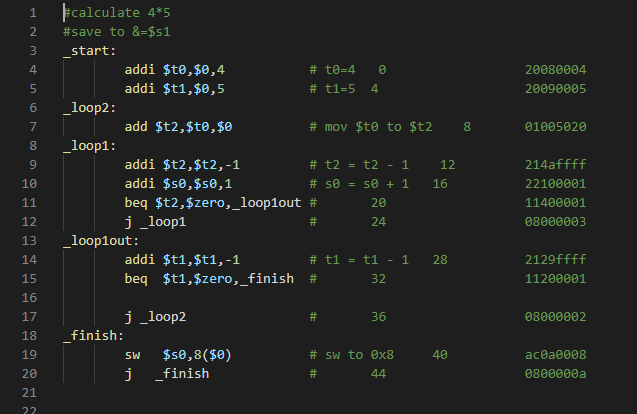
\includegraphics[width=\linewidth]{asm_predictor.png}
	\label{asm_predictor}
\end{figure}


\end{document}






